% !TeX document-id = {ee196d1e-6108-43df-9847-6bc01d26e886}
% !TeX TXS-program:pdflatex = pdflatex -synctex=1 -interaction=nonstopmode --shell-escape %.tex
\documentclass[12pt]{report}
\usepackage[utf8]{inputenc}
%\usepackage[14pt]{extsizes}
\usepackage{listings}
\usepackage{indentfirst}
\usepackage{geometry}
\usepackage{textcomp}
\usepackage{amssymb}
\usepackage{amsmath}
\usepackage{amsthm} 
\usepackage{caption}
\usepackage{misccorr}
\usepackage[noadjust]{cite}
\usepackage{cmap} 
\usepackage[T2A]{fontenc}
\usepackage[english, russian]{babel}
\usepackage{graphics}
\usepackage{graphicx}
\usepackage{textcomp}
\usepackage{verbatim}
\usepackage{makeidx}
\usepackage{float}
\usepackage{bm}
\usepackage{esint}
\usepackage{mathtools}
\usepackage{graphicx}
\usepackage{listings}
% Для листинга кода:
\lstset{ %
language=python,                 % выбор языка для подсветки (здесь это С)
basicstyle=\small\sffamily, % размер и начертание шрифта для подсветки кода
numbers=left,               % где поставить нумерацию строк (слева\справа)
numberstyle=\tiny,           % размер шрифта для номеров строк
stepnumber=1,                   % размер шага между двумя номерами строк
numbersep=5pt,                % как далеко отстоят номера строк от подсвечиваемого кода
showspaces=false,            % показывать или нет пробелы специальными отступами
showstringspaces=false,      % показывать или нет пробелы в строках
showtabs=false,             % показывать или нет табуляцию в строках
frame=single,              % рисовать рамку вокруг кода
tabsize=2,                 % размер табуляции по умолчанию равен 2 пробелам
captionpos=t,              % позиция заголовка вверху [t] или внизу [b] 
breaklines=true,           % автоматически переносить строки (да\нет)
breakatwhitespace=false, % переносить строки только если есть пробел
escapeinside={\#*}{*)}  % если нужно добавить комментарии в коде
}


% plot
\usepackage{pgfplots}
\usepackage{filecontents}
\usetikzlibrary{datavisualization}
\usetikzlibrary{datavisualization.formats.functions}

% Для измененных титулов глав:
\usepackage{titlesec, blindtext, color} % подключаем нужные пакеты
\definecolor{gray75}{gray}{0.75} % определяем цвет
\newcommand{\hsp}{\hspace{20pt}} % длина линии в 20pt
% titleformat определяет стиль
\titleformat{\chapter}[hang]{\Huge\bfseries}{\thechapter\hsp\textcolor{gray75}{|}\hsp}{0pt}{\Huge\bfseries}

\makeatletter
\def\@biblabel#1{#1. }
\makeatother

\usepackage{hyperref}

\newcommand{\specchapter}[1]{\chapter*{#1}\addcontentsline{toc}{chapter}{#1}}
\newcommand{\specsection}[1]{\section*{#1}\addcontentsline{toc}{section}{#1}}
\newcommand{\specsubsection}[1]{\subsection*{#1}\addcontentsline{toc}{subsection}{#1}}

% геометрия
\geometry{pdftex, left = 2cm, right = 2cm, top = 2.5cm, bottom = 2.5cm}

\titlespacing{\chapter}{0pt}{-30pt}{20pt}

\setcounter{tocdepth}{4} % фикс переноса 
\righthyphenmin = 2
\tolerance = 2048

\begin{document}
%\def\chaptername{} % убирает "Глава"
\thispagestyle{empty}
\renewcommand\bibname{Список литературы}

\vspace{\baselineskip}
\noindent \begin{minipage}{0.15\textwidth}
	
\includegraphics[width=\linewidth]{bmstu}
\end{minipage}
\noindent\begin{minipage}{0.9\textwidth}
	\centering
	\textbf{Министерство науки и высшего образования Российской Федерации}\\
	\textbf{Федеральное государственное бюджетное образовательное учреждение высшего образования}\\
	\textbf{«Московский государственный технический университет имени Н.Э.~Баумана}\\
	\textbf{(национальный исследовательский университет)»}\\
	\textbf{(МГТУ им. Н.Э.~Баумана)}
\end{minipage}

\noindent\rule{18cm}{3pt}
\newline\newline
\noindent ФАКУЛЬТЕТ $\underline{\text{«Информатика и системы управления»}}$ \newline\newline
\noindent КАФЕДРА $\underline{\text{«Программное обеспечение ЭВМ и информационные технологии»}}$\newline\newline\newline\newline\newline\newline\newline


\begin{center}
\Large\textbf{Лабораторная работа № 5}
\end{center}
\vspace{\baselineskip}
\noindent\textbf{Дисциплина} $\underline{\text{Анализ алгоритмов~~~~~~~~~~~~~~~~~~~~~~~~~~~~~~~}}$\newline\newline
\noindent\textbf{Тема} $\underline{\text{Конвейерные алгоритмы~~~~~~~~~~~~~~~~~~~~~~~~~~~~~~~~~~~}}$\newline\newline
\noindent\textbf{Студент} $\underline{\text{Искакова К.М.~~~~~~~~~~~~~~~~~~~~~~~~~~~~~~~~~~~~~~~~~~~~}}$\newline\newline
\noindent\textbf{Группа} $\underline{\text{ИУ7-52Б~~~~~~~~~~~~~~~~~~~~~~~~~~~~~~~~~~~~~~~~~~~~~~~~~~~~~~}}$\newline\newline
\noindent\textbf{Оценка (баллы)} $\underline{\text{~~~~~~~~~~~~~~~~~~~~~~~~~~~~~~~~~~~~~~~~~~~~~~~~~~~~~}}$\newline\newline
\noindent\textbf{Преподаватель} $\underline{\text{Волкова Л. Л.~~~~~~~~~~~~~~~~~~~~~~~~~~~~~~~~~~~}}$\newline

\begin{center}
	\vfill
	Москва~---~\the\year
	~г.
\end{center}
\clearpage

\addto{\captionsrussian}{%
	\renewcommand{\contentsname}{\Large{\hspace*{6cm}Содержание}}}%
\renewcommand\contentsname{Содержание}

\tableofcontents

\newpage
\chapter*{Введение}
\addcontentsline{toc}{chapter}{Введение}

Термин «конвейер» пришёл из промышленности, где используется подобный принцип работы — материал автоматически подтягивается по ленте конвейера к рабочему, который осуществляет с ним необходимые действия, следующий за ним рабочий выполняет свои функции над получившейся заготовкой, следующий делает ещё что-то. Таким образом, к концу конвейера цепочка рабочих полностью выполняет все поставленные задачи, сохраняя высокий темп производства. Например, если на самую медленную операцию затрачивается одна минута, то каждая деталь будет сходить с конвейера через одну минуту. В процессорах роль рабочих исполняют функциональные модули, входящие в состав процессора.

В данной лабораторной работе рассматривается конвейерный алгоритм нахождения количества вхождений каждого символа в наборе строк, представленный в двух вариантах: с использованием многопоточности и без.

\vspace{\baselineskip}

\textbf{Задачи работы:}
\begin{enumerate}
	\item рассмотрение стандартного и многопоточного алгоритма нахождения количества вхождений каждого символа в наборе строк;
	\item проведение сравнительного анализа двух реализаций алгоритма;
	\item описание и обосноване полученных результатов.
\end{enumerate}

В ходе лабораторной работы будут изучены возможности конвейерных вычислений и использование подобного подхода на практике.

\chapter{Аналитическая часть}

В  данном  разделе  будет  расмотрена  теоретическая  часть  алгоритма  подсчёта  количе— ства  
вхождений  каждого  символа  в наборе  строк  и теоретические  основы  параллельного 
программирования.

\section{Описание конвейерного алгоритма  без  многопоточности}

Пусть  дана  следующая  последовательность строк,  длина  последовательности —  n.
Для  того,  чтобы  подсчитать  количество  вхождений  каждого  символа  в  каждой  строке, 
необходимо  создать  n  дополнительных массивов,  каждый  из которых  имеет  размерность m,  где:
\begin{itemize}
	\item  n  –  количество  строк  в  исходной  последовательности;
	\item m – мощность  некого  алфавита,  на  основе  которого  строятся  строки.
\end{itemize}

Далее  необходимо  проитерировать  каждую  из  строк  и  инкрементировать  соответствую—
щую  ячейку  массива.
Пример:

\begin{center}
	strings\{"abcd", "defd", "hiji", "kl"\}
\end{center}

Условимся, что все строки составляются из английских строчных букв, таким образом мощностб алфавита $= 26$.

Дополнительные массивы:
\begin{center}
	arr1 = [26];
	
	arr2 = [26];
	
	arr3 = [26];
	
	arr4 = [26];
\end{center}

Допустим,   что  количество  лент $= 2$.  Кaждая из лент  дoлжна  обработать
свою часть.

Так  как  ленты  2,  то каждьая  дoлжна  обработать  по  половине  каждой 
строки.

\begin{center}
	\textbf{Лента 1:}
	
	\vspace{\baselineskip}
	
	"abcd"
	
	arr1['a'] = arr1['a'] + 1
	
	arr1['b'] = arr1['b'] + 1
	
	\vspace{\baselineskip}
	
	"defd"
	
	arr2['a'] = arr2['d'] + 1
	
	arr2['e'] = arr2['e'] + 1
	
	\vspace{\baselineskip}
	\vspace{\baselineskip}
	
	"hiji"
	
	arr3['h'] = arr3['h'] + 1
	
	arr3['i'] = arr3['i'] + 1
	
	\vspace{\baselineskip}

	"kl"
	
	arr4['k'] = arr4['k'] + 1
	
	\vspace{\baselineskip}
	
	\textbf{Лента 2:}
	
	\vspace{\baselineskip}
	
	"abcd"
	
	arr1['c'] = arr1['c'] + 1
	
	arr1['d'] = arr1['d'] + 1
	
	\vspace{\baselineskip}
	
	"defd"
	
	arr2['f'] = arr2['f'] + 1
	
	arr2['d'] = arr2['d'] + 1
	
	\vspace{\baselineskip}
	
	"hiji"
	
	arr3['j'] = arr3['j'] + 1
	
	arr3['i'] = arr3['i'] + 1
	
	\vspace{\baselineskip}
	
	"kl"
	
	arr4['l'] = arr4['l'] + 1
\end{center}

Таким  образом  на  выходе  получаем  следующие  значения:

\begin{center}
arr1[’а’] = 1

arr1[’b’] = 1

arr1[’с’] = 1

arr1[’d'] = 1

arr2[’d'] = 2

arr2[’е'] = 1

arr2[’f'] = 1

агг3[’h'] = 1

агг3[’i’] = 1

агг3[’ј'] = 2

arr4[’k'] = 1

arr4[’l’] = 1
\end{center}

Все остальные  ячейки  равны  нулю.

Таким образом, в каждом из соответствующих массивов хранится количество вхождений каждого из символов алфавита в соответствующей строке.

\section{Описание конвейерного алгоритма  с использованием  многопоточности}

В целом алгоритм,  в основе которого  лежит использование  множества  потоков  является схожим с 
последовательным алгоритмом  с той лишь разницей,  что потоки делят между собой  адресное  
пространство.  Таким  образом,  в отличие  от  последовательного алгоритма мoжнo  не  дожидаться  
пока  каждьiй  из  конвейеров  обработает  \textbf{все}   строки,  а  передавать \textbf{yжe    обработанные}  строки 
на обработку  следующему  конвейеру.

\section{Параллельное программирование}

При использовании многопроцессорных вычислительных систем с общей памятью обычно предполагается, что имеющиеся в составе системы процессоры обладают равной производительностью, являются равноправными при доступе к общей памяти, и время доступа к памяти является одинаковым (при одновременном доступе нескольких процессоров к одному и тому же элементу памяти очередность и синхронизация доступа обеспечивается на аппаратном уровне). Многопроцессорные системы подобного типа обычно именуются симметричными мультипроцессорами (symmetric multiprocessors, SMP) \cite{tri}.

Обычный подход при организации вычислений для многопроцессорных вычислительных систем с общей памятью – создание новых параллельных методов на основе обычных последовательных программ, в которых или автоматически компилятором, или непосредственно программистом выделяются участки независимых друг от друга вычислений. Возможности автоматического анализа программ для порождения параллельных вычислений достаточно ограничены, и второй подход является преобладающим.

Широко используемый подход состоит и в применении тех или иных библиотек, обеспечивающих определенный программный интерфейс (application programming interface, API) для разработки параллельных программ. В рамках такого подхода наиболее известны Windows Thread API \cite{odin}. Однако первый способ применим только для ОС семейства Microsoft Windows, а второй вариант API является достаточно трудоемким для использования и имеет низкоуровневый характер.

\section{Организация взаимодействия параллельных потоков}

Как  yжe  было  сказано,  потоки,  в  отличии  от  процессов,   не  имеют  собственного   адресного  пространства.   Как   результат,   взаимодействи  потоков  мoжнo  реализовать   через 
использование  общих  данных.  В  случае,  когда общие  данные  необходимо  только  читать  — 
проблем  возникнуть  не мoжeт.  В  случае,  если необходимо  общие  данные  изменять  —  необходимо  пользоваться  средствами  синхронизации:  mutex,  семафор.

\section{Вывод}

В данном разделе была рассмотрена теоритическая часть конвейерного  алгоритма  по— иска  
вхождения  символа  в  каждой  из  строк  из  набора  строк,  а  тaкиe  описаны  две  его 
реализации:  с  использованием многопоточности  и без.  Была  рассмотрена  технология параллельного программирования и организация взаимодействия параллелных потоков.

Также предоставим к ПО следующие требования:

\textbf{Требования  к  вводу:}  на вход подаётся  количество  строк  и сами строки.

\textbf{Требования  к  программе:}  Подсчёт  количества  вхождений  каждого  символа  в каждой строке.


\chapter{Конструкторская часть}
В этом разделе содержатся cхемы реализуемых алгоритмов.

На вход алгоритм принимает количество строк и сами строки.
	
\section{Схемы алгоритмов}
На Рис. 2.1–2.2 представлена схема последователного конвейерного алгоритма подсчета.

\vspace{\baselineskip}

\begin{figure}[h]
	\center{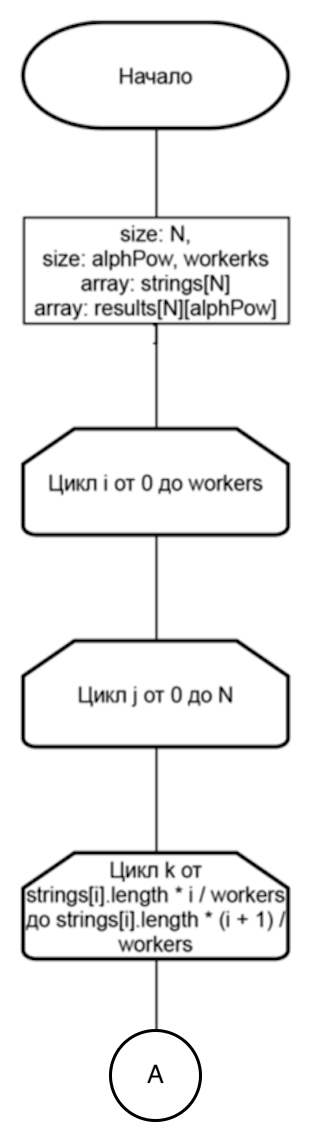
\includegraphics[scale=0.4]{alg1-1}}
	\caption{Схема последователного конвейерного алгоритма подсчета. Часть 1.}
	\label{figure:image}
\end{figure}

\begin{figure}[h!]
	\center{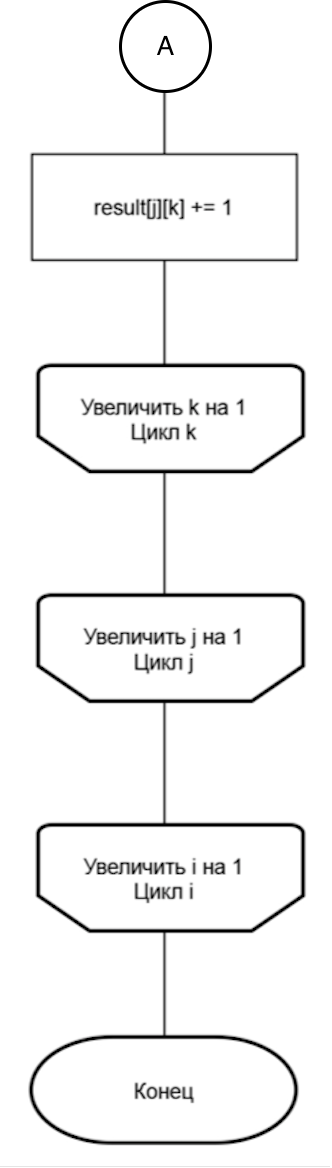
\includegraphics[scale=0.4]{alg1-2}}
	\caption{Схема последователного конвейерного алгоритма подсчета. Часть 2.}
	\label{figure:image}
\end{figure}

\clearpage

\begin{figure}[h]
На Рис. 2.3 представлена схема главного потока параллельного конвейерного алгоритма.
\end{figure}

\begin{figure}[h!]
	\center{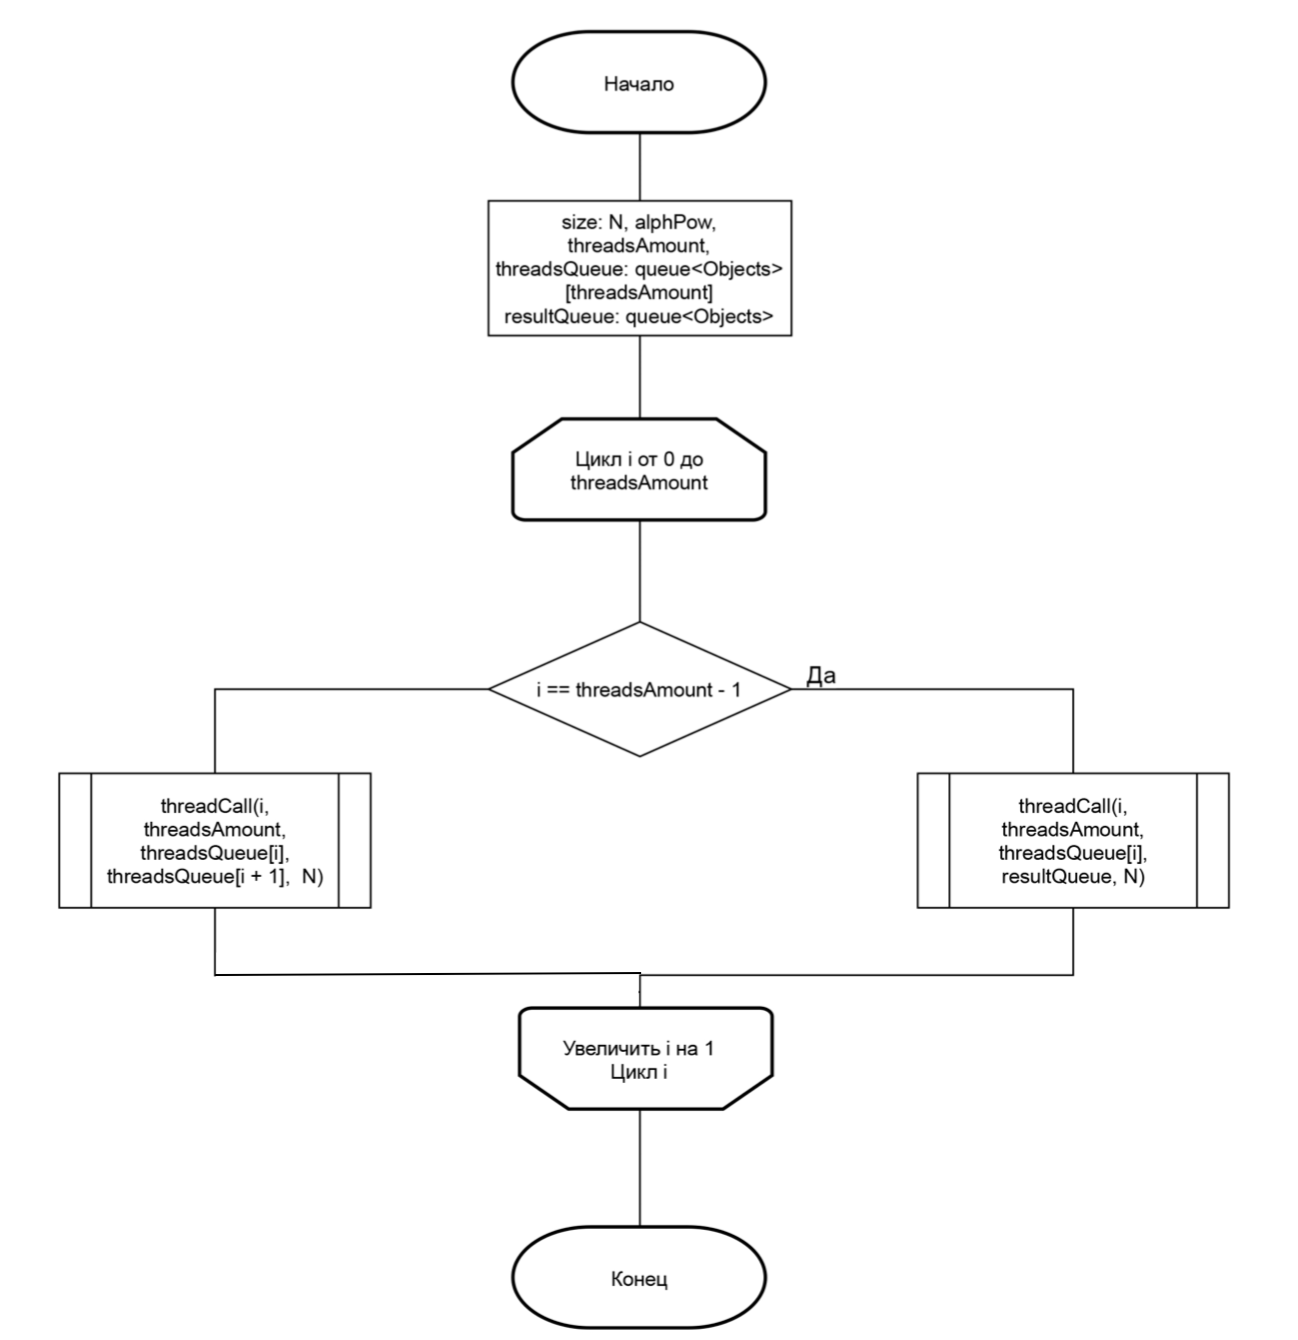
\includegraphics[scale=0.8]{alg2}}
	\caption{Схема главного потока параллельного конвейерного алгоритма.}
	\label{figure:image}
\end{figure}

\clearpage

\begin{figure}[h!]
	На Рис. 2.4-2.5 представлена схема дочернего потока параллельного конвейерного алгоритма.
\end{figure}

\begin{figure}[h!]
	\center{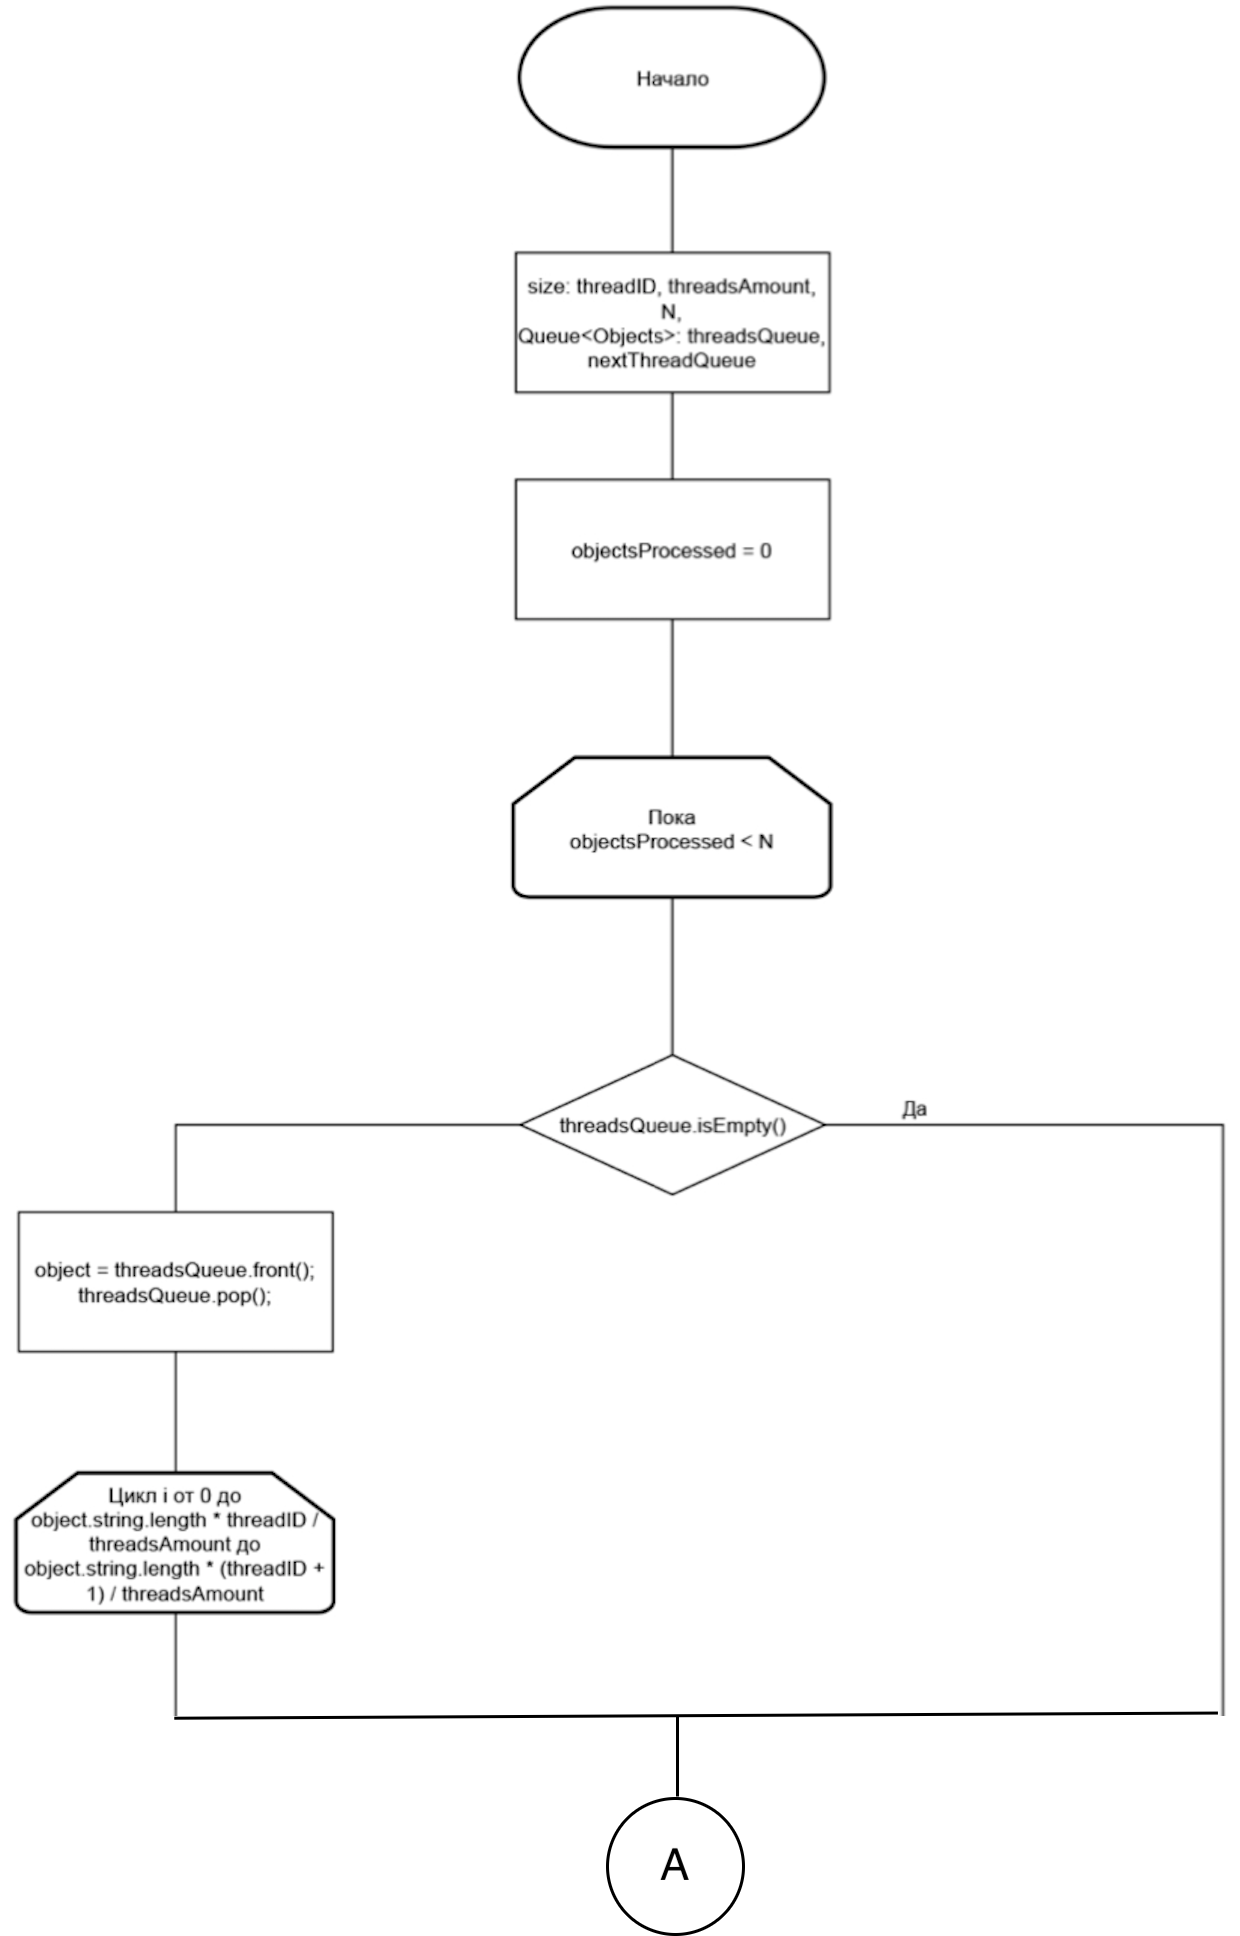
\includegraphics[scale=0.25]{alg3-1}}
	\caption{Схема дочернего потока параллельного конвейерного алгоритма. Часть 1.}
	\label{figure:image}
\end{figure}

\begin{figure}[h!]
	\center{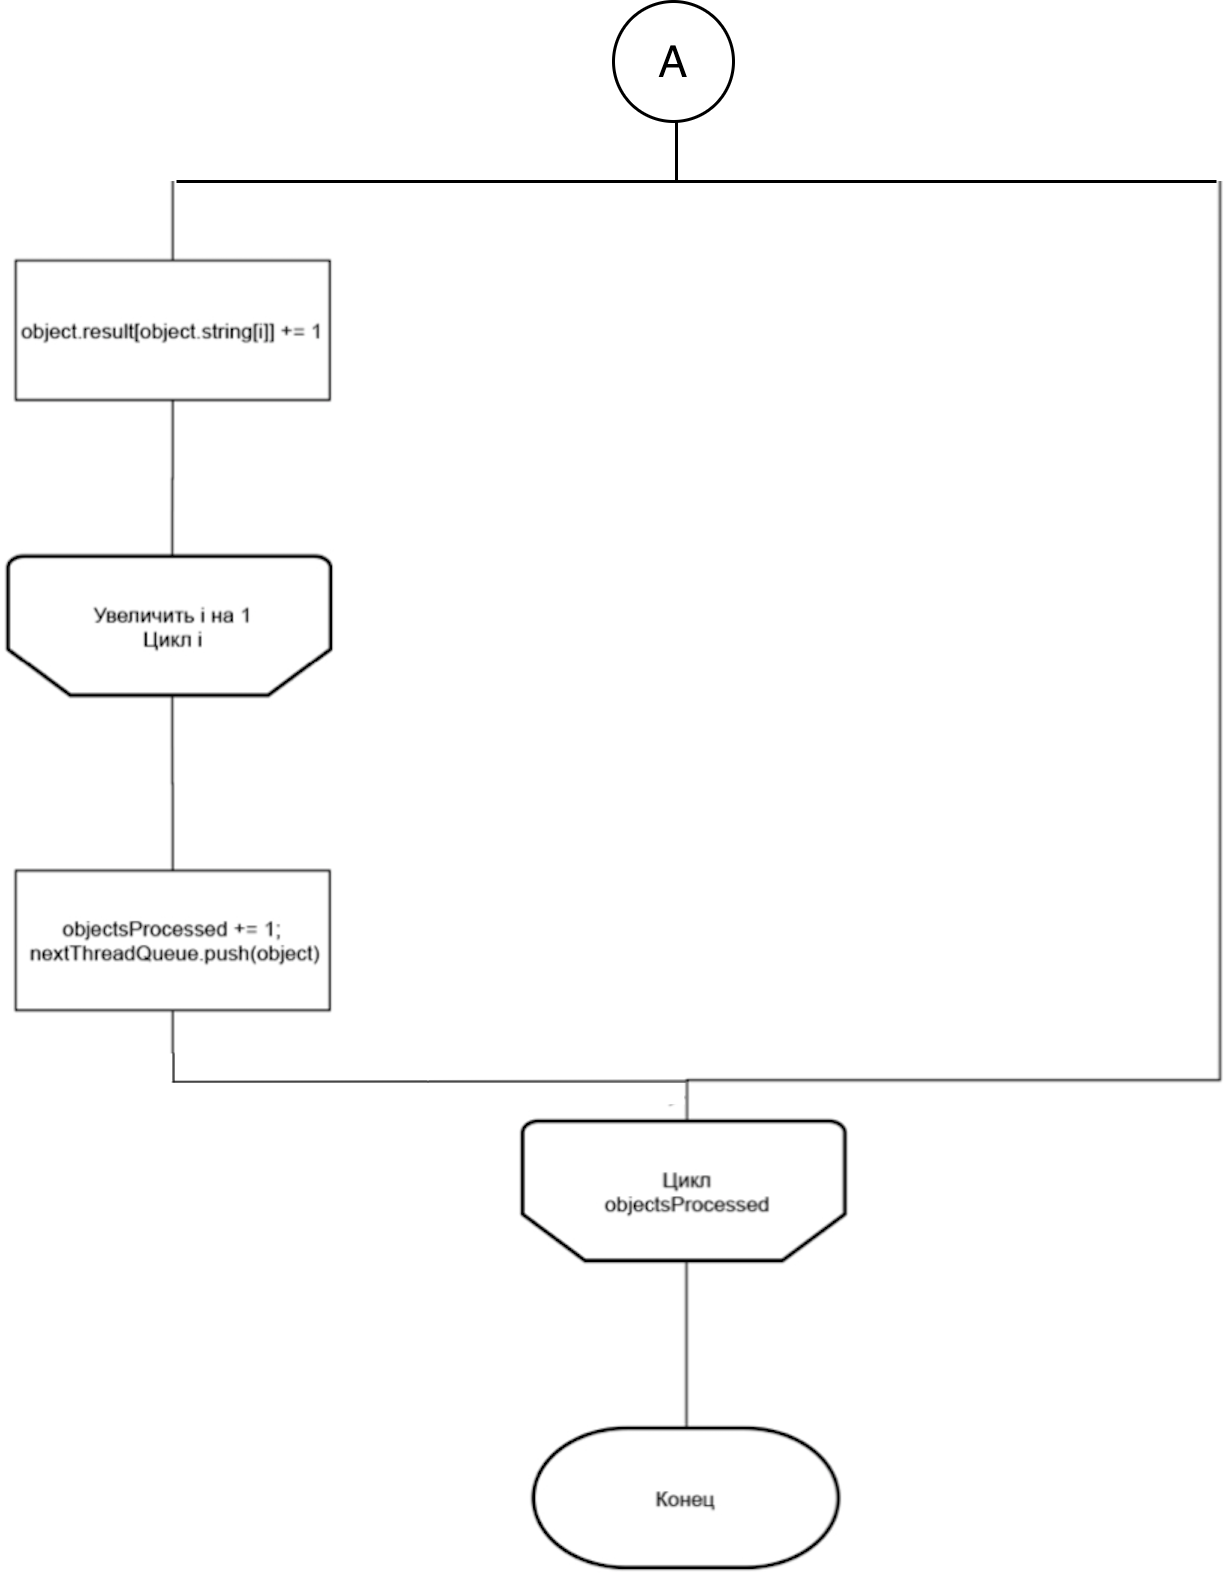
\includegraphics[scale=0.3]{alg3-2}}
	\caption{Схема дочернего потока параллельного конвейерного алгоритма. Часть 2.}
	\label{figure:image}
\end{figure}

\chapter{Технологическая часть}
В данном разделе будут рассмотрены требования к программному обеспечению, средства реализации, представлен листинг кода и описание тестирования.

\section{Средства реализации}
В качестве языка программирования был выбран С++ т.к. я знакома с данным языком, у него есть уникальный баланс между возможностями объектно-ориентированного программирования и производительностью. Он одновременно позволяет писать высокоуровневый абстрактный код, который при этом работает со скоростью близкой к машинному коду.

Среда разработки — CLion, которая предоставляет умную проверку кода, быстрое выявление ошибок и оперативное исправление, вкупе с автоматическим рефакторингом кода, и богатыми возможностями в навигации.  

Время работы алгоритмов было замерено с помощью функции steady\_clock() из библиотеки chrono \cite{chrono}. 

Для тестирования использовался компьютер на базе процессора 2,2 GHz Intel Core i7 \cite{intel}, 6 ядер, 4 логических процессора

\newpage
\section{Листинг кода}

В Листинге 3.1 показана реализация последовательного алгоритма подсчета.

\begin{flushleft}
Листинг 3.1. Последовательный алгоритм подсчета.
\begin{lstlisting}
static void countLettersInObject (WorkObject& object, size_t startLetter, size_t endLetter) 
{
		for (size_t i = startLetter; i < endLetter; i++) 
		{
				object.result[object.string[i] - 'a']++;
		}
}

void linearWorker(std::queue<WorkObject>& objects, 	
								const size_t workerNumber, 
								const size_t workersAmount, 
								size_t elementsToProcess) 
{
		for (size_t i = 0; i < elementsToProcess; i++) 
		{
				WorkObject object = objects.front();
				objects.pop();
				countLettersInObject(object,
													  object.string.length() * (double)workerNumber / workersAmount,
													  object.string.length() * (double)(workerNumber + 1) / workersAmount);
				objects.push(object);
		}
}

std::vector<WorkObject> initLinearWork(std::vector<std::string>& strings, 
						  const int workersAmount) 
{
		std::queue<WorkObject> objects;
		for (auto& string : strings) 
		{
			objects.emplace(WorkObject(string));
		}
		MyTimer Timer;
		for (int i = 0; i < workersAmount; i++) 
		{
			linearWorker(objects, i, workersAmount, strings.size());
		}
		std::cout << "Linear alg works for: " << 
							  Timer.elapsed() << 
							  " seconds" << std::endl;
		std::vector<WorkObject> result;
		while (!objects.empty()) 
		{
			result.push_back(objects.front());
			objects.pop();
		}
		return result;
}
\end{lstlisting}
\end{flushleft}

\vspace{\baselineskip}

В Листинге 3.2 показана реализация главного потока параллельного конвейерного алгоритма подсчета.

\begin{flushleft}
Листинг 3.2. Главный поток параллельного конвейерного алгоритма подсчета.
\begin{lstlisting}
std::vector<WorkObject> initConveyorWork(std::vector<std::string>& strings, const int workersAmount) {
	std::queue<WorkObject> completedObjects;
	std::vector<std::queue<WorkObject>> workersQueues(workersAmount);
	std::vector<std::thread> threads;
	for (auto& string : strings) {
		workersQueues[0].push(WorkObject(string));
	}
	
	std::vector<std::mutex> mutexes(workersAmount + 1);
	
	MyTimer timerAllWork;
	for (size_t i = 0; i < workersAmount; i++) {
		threads.emplace_back(std::thread(threadWork, i, workersAmount, std::ref(workersQueues[i]),
		i == workersAmount - 1 ? std::ref(completedObjects) : std::ref(
		workersQueues[i + 1]), strings.size(), std::ref(mutexes[i]),
		std::ref(mutexes[i + 1])));
	}
	
	for (size_t i = 0; i < workersAmount; i++) {
		threads[i].join();
	}
	
	std::cout << "All Conveyor worked for: " << timerAllWork.elapsed() << " seconds" << std::endl;
	std::vector<WorkObject> result;
	while (!completedObjects.empty()) {
		result.push_back(completedObjects.front());
		completedObjects.pop();
	}
	return result;
}
\end{lstlisting}
\end{flushleft}

В Листинге 3.3 представлена реализация дочернего потока параллельного конвейерного алгоритма подсчета.
.
\begin{flushleft}
Листинг 3.3. Дочерний поток параллельного конвейерного алгоритма подсчета.
\begin{lstlisting}
static void countLettersInObject (WorkObject& object, size_t startLetter, size_t endLetter) {
	for (size_t i = startLetter; i < endLetter; i++) {
		object.result[object.string[i] - 'a']++;
	}
}

std::mutex allThreadsLock;

void threadWork(const int threadNumber, const int threadsAmount, std::queue<WorkObject>& threadsQueue, std::queue<WorkObject>& nextThreadQueue, size_t objectsToProcess,
std::mutex& threadsMutex, std::mutex& nextThreadsMutex) {
	MyTimer timerThreadWork;
	size_t sleepTime;
	size_t processed = 0;
	while(processed != objectsToProcess) {
		if (threadsQueue.size()) {
			WorkObject object = threadsQueue.front();
			
			threadsMutex.lock();
			threadsQueue.pop();
			threadsMutex.unlock();
			
			countLettersInObject(object, object.string.length() * (double)threadNumber / threadsAmount, object.string.length() * (double)(threadNumber + 1) / threadsAmount);
			
			nextThreadsMutex.lock();
			nextThreadQueue.push(object);
			nextThreadsMutex.unlock();
			
			processed++;
		} else {
			usleep(1000);
			sleepTime += 1;
		}
	}
	
	allThreadsLock.lock();
	std::cout << "Thread # " << threadNumber << " worked for " << timerThreadWork.elapsed() << " seconds" << std::endl;
	std::cout << "Thread # " << threadNumber << " sleeped for " << sleepTime << " milliseconds" << std::endl;
	allThreadsLock.unlock();
}
\end{lstlisting}
\end{flushleft}
	
\section{Тестирование}
Были проведены тесты на больших размерностях со случайными строками в качестве элементов.
\vspace{\baselineskip}

На листинге 3.4 представлен фрагмент кода тестирования корректной работы реализации алгоритмов.

\begin{flushleft}
Листинг 3.4. Тестирование корректной работы алгоритмов.
\begin{lstlisting}
int tests(size_t wordsAmount, size_t lettersInWord) 
{
	std::vector<std::string> strings;
	for (size_t i = 0; i < wordsAmount; i++) 
	{
		std::string string;
		for (size_t j = 0; j < lettersInWord; j++) 
		{
			string.push_back(rand() % LETTERS_IN_ENG_ALPHABET + 'a');
		}
		strings.emplace_back(string);
	}
	
	std::vector<WorkObject>  resultConsistent = initLinearWork(strings, 3);
	
	std::vector<WorkObject>  resultConveyor = initConveyorWork(strings, 3);
	
	if (resultConsistent != resultConveyor)
	{
		return EXIT_FAILURE;
	}
	
	return EXIT_SUCCESS;
}
\end{lstlisting}
\end{flushleft}

Все тесты пройдены успешно.

\chapter{Экспериментальная часть}

В данном разделе приведен анализ алгоритмов на основе эксперементальных данных.

\section{Сравнительный анализ на основе замеров времени работы алгоритмов} 

Был  проведён  замер  времени  работы  каждого  из  параллельных   алгоритмов.   Длина каждой  
строки  10000  символов.   Каждый  эксперимент  на  каждой  размерности  массива строк  был 
произведён  5 раз,  затем  бралось  среднее  арифметическое полученного  результата.

Для всех  замеров  количество  лент $= 3$.
Во всех  таблицах  время  выполнения  указано в секундах.

В  таблице  4.1  показаны  результаты  замеров  выполнения  программы  для 
последовательной и параллельной  реализаций  соответственно.

\begin{figure}[h!]
	\center{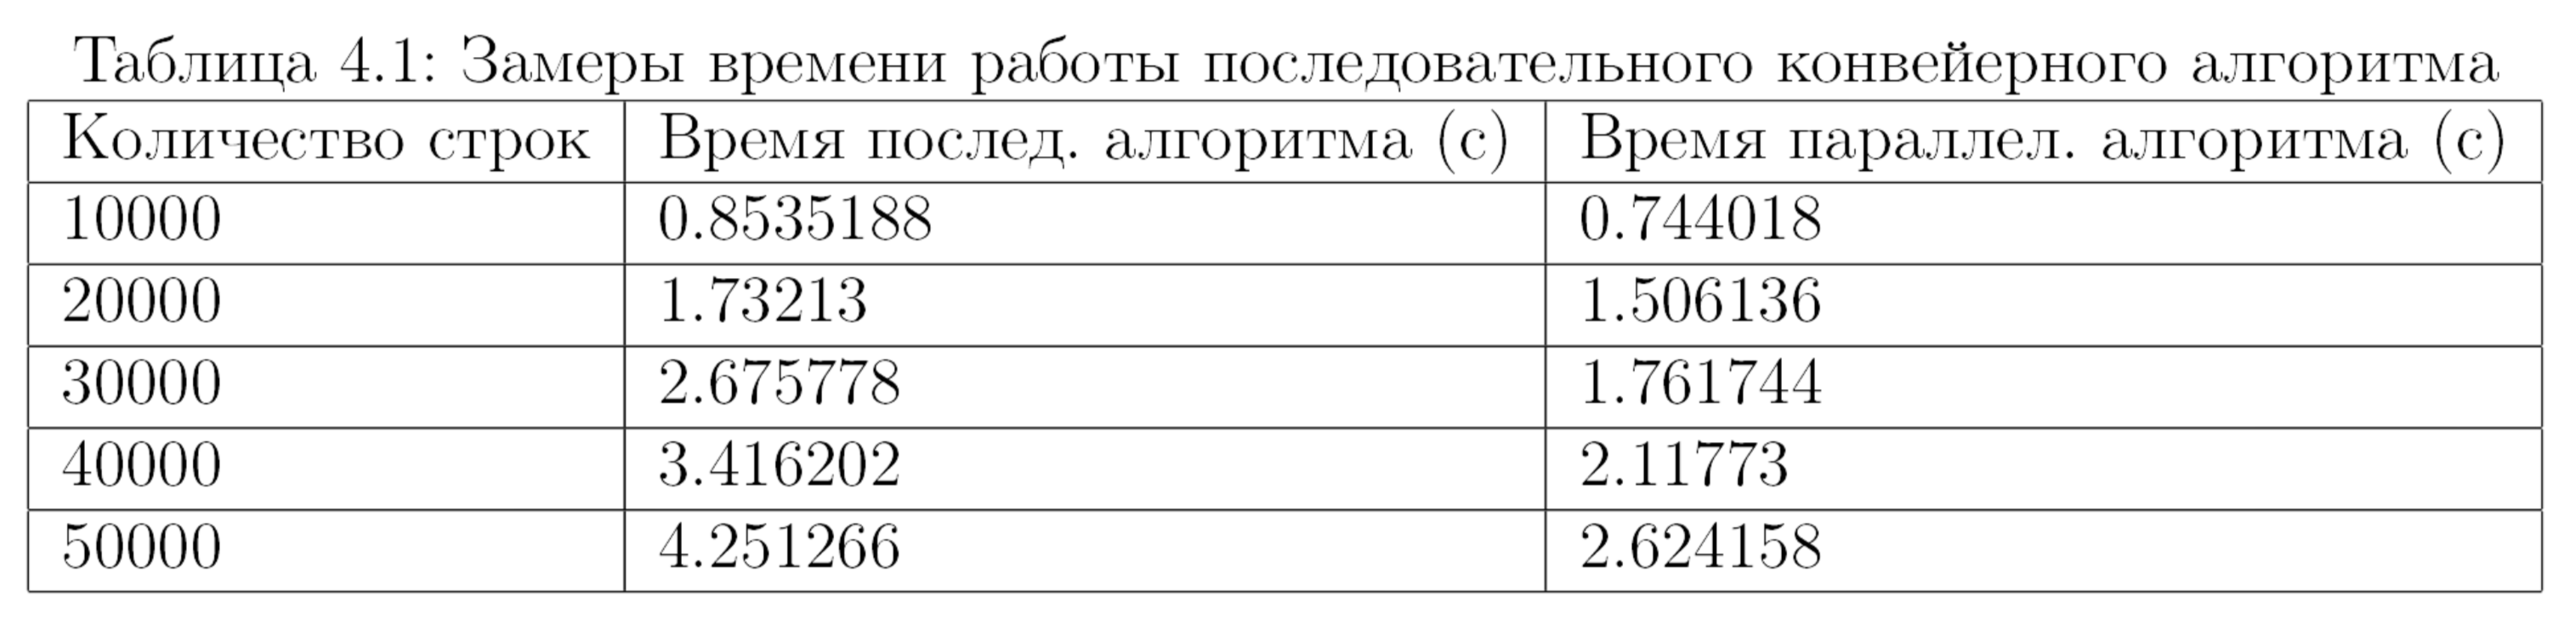
\includegraphics[scale=0.3]{table1}}
	\label{figure:image}
\end{figure}

Ниже,  на рисунке  4.1,  показана  графическая  интерпретация  таблицы  4.1

\begin{figure}[h!]
	\center{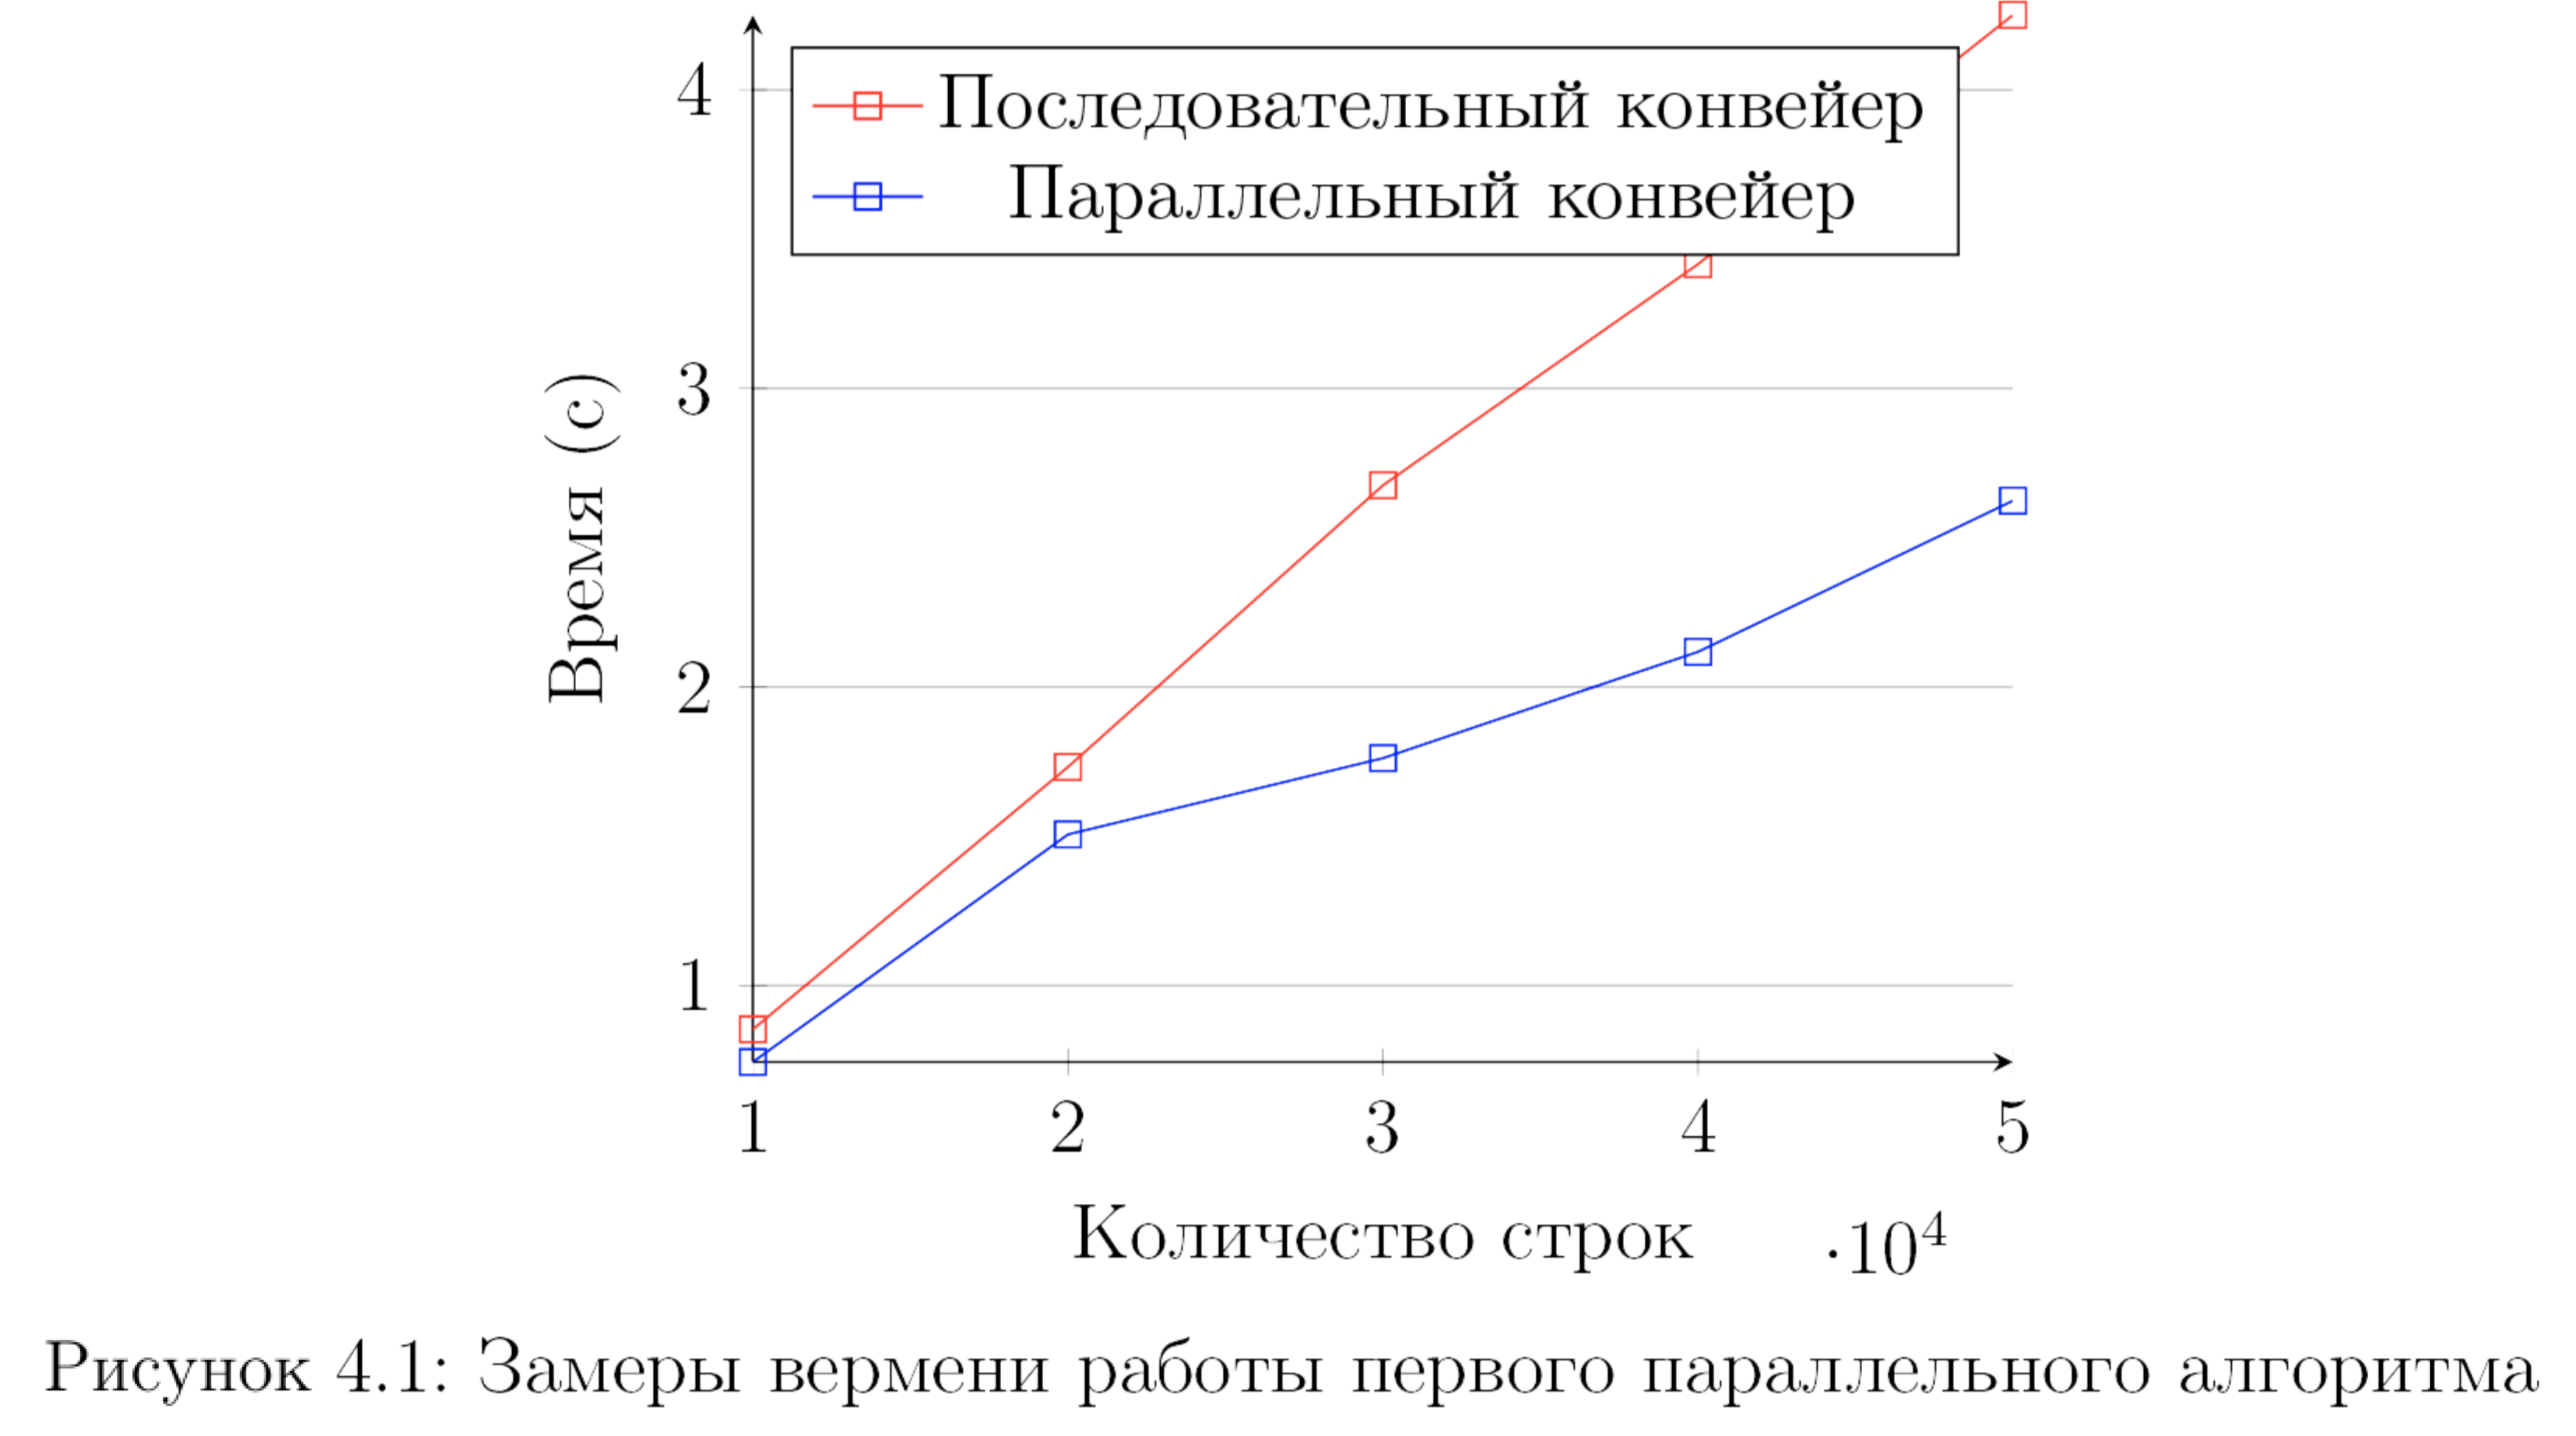
\includegraphics[scale=0.3]{graph1}}
	\label{figure:image}
\end{figure}
 
 \section*{Вывод}
 \qquad По результатам исследования получилось, что при малых размерностях входных данных разница по времени между алгоритмами не существенна, но с увеличением размерности эффективнее использовать параллельный алгоритм подсчета.
 
\newpage
\chapter*{Заключение}
\addcontentsline{toc}{chapter}{Заключение}
\hspace{0.6cm}В ходе лабораторной работы был изучен алгоритм нахождения количеста вхождений каждого символа в наборе строк, а также разработаны 2 конвейерные версии этого алгоритма: последовательный и параллельный. Эксперементально было установлено, что параллельные версии быстрее последовательного алгоритма.


\begin{thebibliography}{2}
	\addcontentsline{toc}{chapter}{Список литературы}
	\bibitem{tri} Богачев К.Ю. Основы параллельного программирования. – М.: БИНОМ. Лаборатория знаний 2003. - 237 с.
	\bibitem{odin} Справка по потокам в ОС Windows [электронный ресурс]. Режим доступа: https://docs.microsoft.com/en-us/windows/win32/procthread/process-and-thread-functions, свободный (дата обращения: 09.12.2021)
	\bibitem{chrono} Официальный сайт Microsoft, документация [электронный ресурс]. Режим доступа: https://docs.microsoft.com/ru-ru/cpp/standard-library/chrono?view=vs-2017, свободный (дата обращения: 09.12.21)
	\bibitem{dva} Кнут Д. Э. Искусство программирования. Том 1. Сортировка и поиск. – М.: Вильямс, 2007. - 832 с.
	\bibitem{intel} Официальный сайт Intel [электронный ресурс]. Режим доступа: https://ark.intel.com/content/www/ru/ru/ark/products/134906/intel-core-i78750h-processor-9m-cache-up-to-4-10-ghz.html, свободный (дата обращения: 09.12.21)
	
\end{thebibliography}
\end{document}